\documentclass{article}
\usepackage[margin=0.75in]{geometry}
\usepackage[utf8]{inputenc}
\usepackage[section]{placeins}
\usepackage{graphicx}
\graphicspath{{./images/}}
\usepackage{float}
\usepackage{listings}
\usepackage{framed}

\title{jRAPL Testing Results}
\author{Alejandro Servetto}
\begin{document}
\maketitle

System C is a Thinkpad E15. My new Computer (describe the rest of the specs...)

\section{UML Class Diagram}
    The UML is too big to fit on a page, but you can see it in the 'img' folder

\section{Async Monitor Comparison (C vs Java)}

\subsection{Explaining why Java was so much faster than C, or so it seems. It was based on the sleep implementation}
    \subsubsection{Sleep implementation}
        In Java, I use \texttt{Thread.sleep(msec)}. In C, I use the following:
        \begin{verbatim}
            int sleep_msec(long msec) {
	            struct timespec ts;
	            int res;

            	if (msec < 0) {
	            	errno = EINVAL;
            		return -1;
            	}

            	ts.tv_sec = msec / 1000;
	            ts.tv_nsec = (msec % 1000) * 1000000;

            	do {
	            	res = nanosleep(&ts, &ts);
	            } while (res && errno == EINTR);
	            
	            return res;
            }
        \end{verbatim}
At 0 ms, the C sleep is on average 52 usec slower than Java. At nonzero sleep rates, its different
    \begin{figure}[H]
    	\centering
    	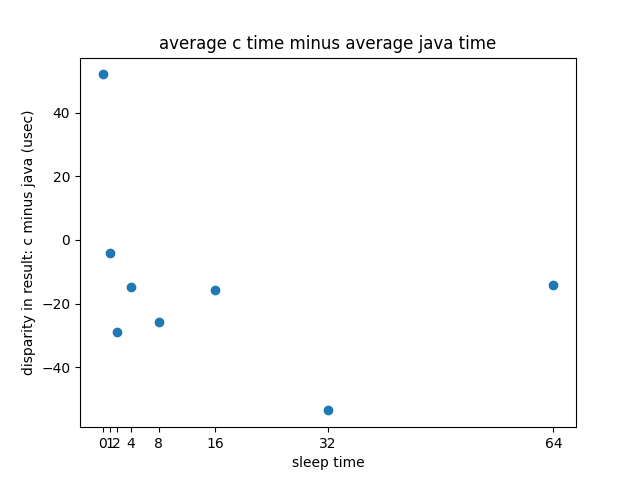
\includegraphics[width=17cm,height=20cm,keepaspectratio]{AsyncMonitorCompares/sleep-timer_java-vs-c/c-java-avg-difference.png}
    	\caption{PKG dacapo results xalan}
    	\label{fig:xalan-fix-PKG}
    \end{figure}
    Comparing time for \{0,1,2,4,8,16,32,64\} milliseconds
    \begin{figure}[H]
    	\centering
    	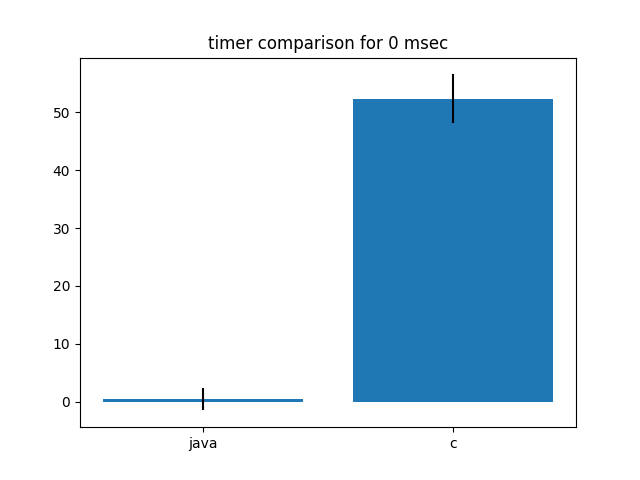
\includegraphics[width=17cm,height=20cm,keepaspectratio]{AsyncMonitorCompares/sleep-timer_java-vs-c/time-compare-0.png}
    	\caption{recorded time to sleep 0 ms}
    	\label{fig:xalan-fix-PKG}
    \end{figure}
    \begin{figure}[H]
    	\centering
    	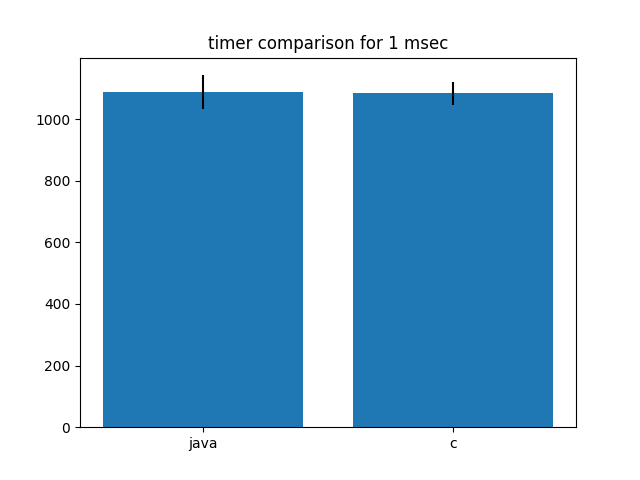
\includegraphics[width=17cm,height=20cm,keepaspectratio]{AsyncMonitorCompares/sleep-timer_java-vs-c/time-compare-1.png}
    	\caption{recorded time to sleep 1 ms}
    	\label{fig:xalan-fix-PKG}
    \end{figure}
    \begin{figure}[H]
    	\centering
    	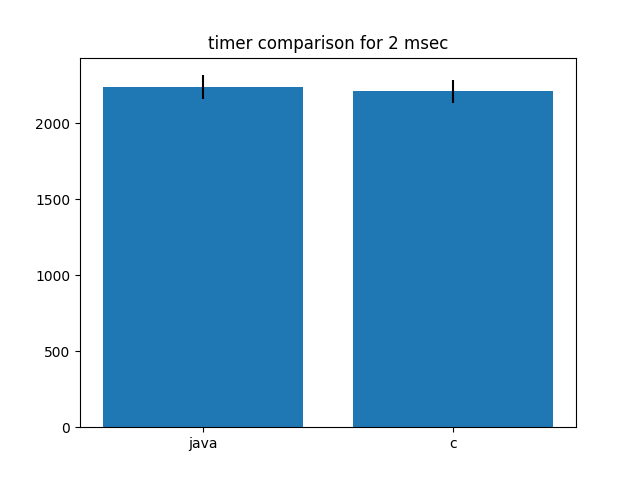
\includegraphics[width=17cm,height=20cm,keepaspectratio]{AsyncMonitorCompares/sleep-timer_java-vs-c/time-compare-2.png}
    	\caption{recorded time to sleep 2 ms}
    	\label{fig:xalan-fix-PKG}
    \end{figure}
    \begin{figure}[H]
    	\centering
    	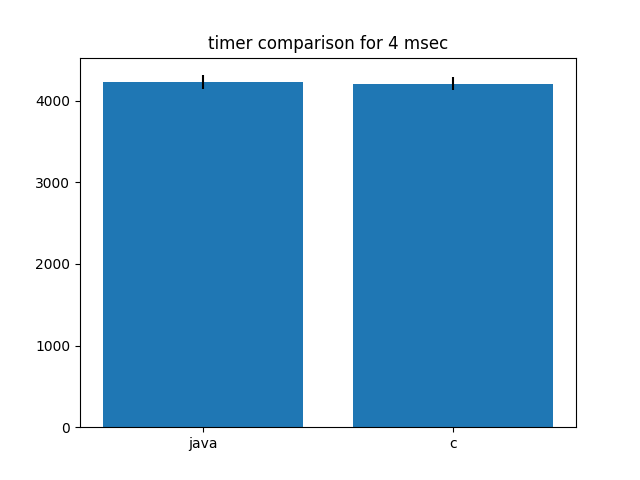
\includegraphics[width=17cm,height=20cm,keepaspectratio]{AsyncMonitorCompares/sleep-timer_java-vs-c/time-compare-4.png}
    	\caption{recorded time to sleep 4 ms}
    	\label{fig:xalan-fix-PKG}
    \end{figure}
    \begin{figure}[H]
    	\centering
    	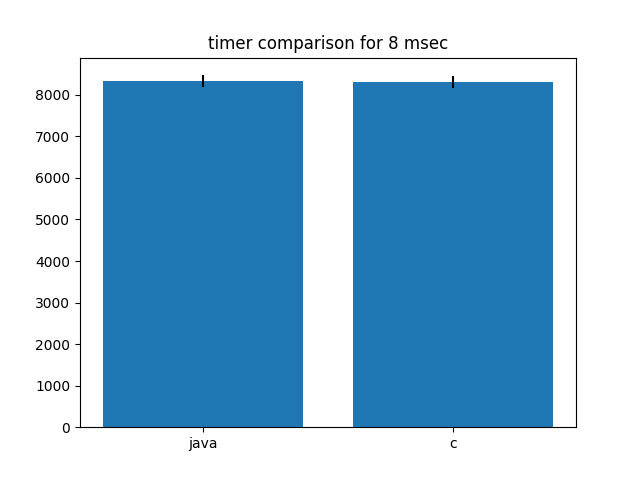
\includegraphics[width=17cm,height=20cm,keepaspectratio]{AsyncMonitorCompares/sleep-timer_java-vs-c/time-compare-8.png}
    	\caption{recorded time to sleep 8 ms}
    	\label{fig:xalan-fix-PKG}
    \end{figure}
    \begin{figure}[H]
    	\centering
    	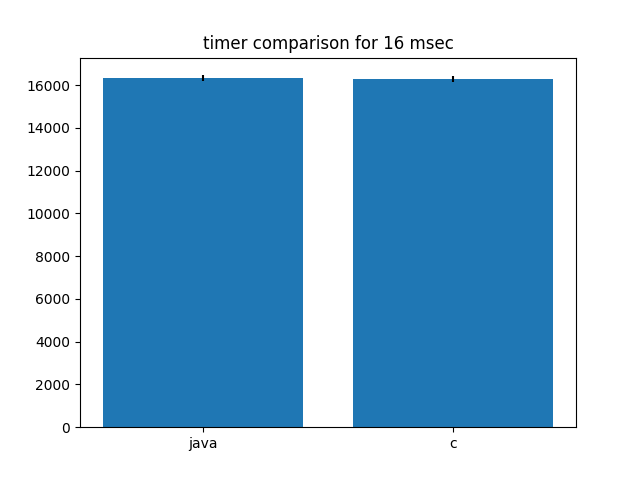
\includegraphics[width=17cm,height=20cm,keepaspectratio]{AsyncMonitorCompares/sleep-timer_java-vs-c/time-compare-16.png}
    	\caption{recorded time to sleep 16 ms}
    	\label{fig:xalan-fix-PKG}
    \end{figure}
    \begin{figure}[H]
    	\centering
    	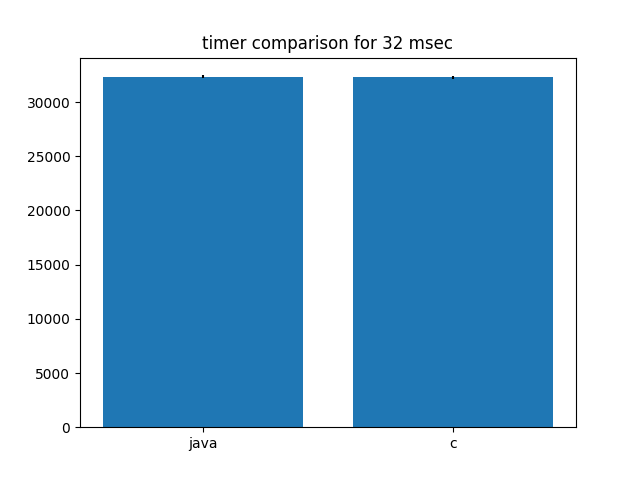
\includegraphics[width=17cm,height=20cm,keepaspectratio]{AsyncMonitorCompares/sleep-timer_java-vs-c/time-compare-32.png}
    	\caption{recorded time to sleep 32 ms}
    	\label{fig:xalan-fix-PKG}
    \end{figure}
    \begin{figure}[H]
    	\centering
    	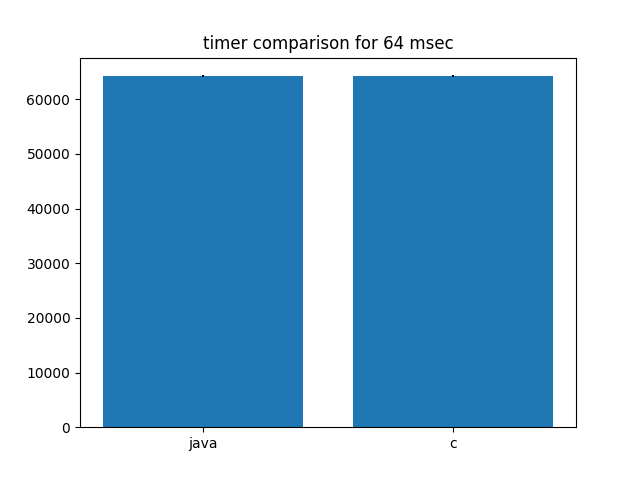
\includegraphics[width=17cm,height=20cm,keepaspectratio]{AsyncMonitorCompares/sleep-timer_java-vs-c/time-compare-64.png}
    	\caption{recorded time to sleep 64 ms}
    	\label{fig:xalan-fix-PKG}
    \end{figure}


\subsection{Tied into Dacapo}
Made a callback harness, start a monitor right before a bench iteration, stop right after. Do 15 iterations, record data for the
latter 10. Experiments in this subsection were run on Jolteon

\subsubsection{Number of samples collected -- 1ms sampling rate}
Looks like C is actually faster than Java! Makes sense, given the JNI overhead difference we measured \textbf{NOTE THAT THIS IS ONLY THE AVERAGE OF 3 ITERS AFTER 1 WARMUP.}. I need to take a few hours to run it when I have the space to do so.

\textbf{Should I do samples / msec? The benchmarks each vary in runtime, which is why bars are longer between benchmarks, not necessarily about the benchmarks themselves}
    \begin{figure}[H]
    	\centering
    	\includegraphics[width=17cm,height=20cm,keepaspectratio]{jolteon/compare-async-monitor/dacapo/num-samples/all-bench_numsamples.png}
    	\caption{Number of samples collected across all benchmarks}
    	\label{fig:xalan-fix-PKG}
    \end{figure}

\subsubsection{Number of samples collected -- 0 sampling rate, probably deprecated since the 0 rate isn't practical because of reasons}
Interestingly enough, Java version collected way more samples in around the same timespan. The plots below are averages
across 10 benchmark iterations. We see that this is consistent for Java across all the used benchmarks. Unless I'm mistaken we also see that the disparity between C versions and Java versions increases the longer the monitor runs (I should make a numeric way to quanitfy
the relationship between disparity and lifetime or something, I'm only going based off of eyeballing the graphs right now.

I intend to see if this is because of the timer implementation different or because of thread scheduling in C vs Java. Was suggested I
look at \texttt{strace} to see if threads behave differently. I started a thing to test the difference between the two timer implementations, although I need to flesh that out better

    \begin{figure}[H]
    	\centering
    	\includegraphics[width=17cm,height=20cm,keepaspectratio]{jolteon/compare-async-monitor/dacapo/num-samples/avrora_numsamples.png}
    	\caption{results for avrora}
    \end{figure}
    \begin{figure}[H]
    	\centering
    	\includegraphics[width=17cm,height=20cm,keepaspectratio]{jolteon/compare-async-monitor/dacapo/num-samples/batik_numsamples.png}
    	\caption{results for batik}
    \end{figure}
    \begin{figure}[H]
    	\centering
    	\includegraphics[width=17cm,height=20cm,keepaspectratio]{jolteon/compare-async-monitor/dacapo/num-samples/biojava_numsamples.png}
    	\caption{results for biojava}
    \end{figure}
    \begin{figure}[H]
    	\centering
    	\includegraphics[width=17cm,height=20cm,keepaspectratio]{jolteon/compare-async-monitor/dacapo/num-samples/cassandra_numsamples.png}
    	\caption{results for cassandra}
    \end{figure}
    \begin{figure}[H]
    	\centering
    	\includegraphics[width=17cm,height=20cm,keepaspectratio]{jolteon/compare-async-monitor/dacapo/num-samples/eclipse_numsamples.png}
    	\caption{results for eclipse}
    \end{figure}
    \begin{figure}[H]
    	\centering
    	\includegraphics[width=17cm,height=20cm,keepaspectratio]{jolteon/compare-async-monitor/dacapo/num-samples/fop_numsamples.png}
    	\caption{results for fop}
    \end{figure}
    \begin{figure}[H]
    	\centering
    	\includegraphics[width=17cm,height=20cm,keepaspectratio]{jolteon/compare-async-monitor/dacapo/num-samples/graphchi_numsamples.png}
    	\caption{results for graphchi}
    \end{figure}
    \begin{figure}[H]
    	\centering
    	\includegraphics[width=17cm,height=20cm,keepaspectratio]{jolteon/compare-async-monitor/dacapo/num-samples/h2_numsamples.png}
    	\caption{results for h2}
    \end{figure}
    \begin{figure}[H]
    	\centering
    	\includegraphics[width=17cm,height=20cm,keepaspectratio]{jolteon/compare-async-monitor/dacapo/num-samples/h2o_numsamples.png}
    	\caption{results for h2o}
    \end{figure}
    \begin{figure}[H]
    	\centering
    	\includegraphics[width=17cm,height=20cm,keepaspectratio]{jolteon/compare-async-monitor/dacapo/num-samples/jme_numsamples.png}
    	\caption{results for jme}
    \end{figure}
    \begin{figure}[H]
    	\centering
    	\includegraphics[width=17cm,height=20cm,keepaspectratio]{jolteon/compare-async-monitor/dacapo/num-samples/jython_numsamples.png}
    	\caption{results for jython}
    \end{figure}
    \begin{figure}[H]
    	\centering
    	\includegraphics[width=17cm,height=20cm,keepaspectratio]{jolteon/compare-async-monitor/dacapo/num-samples/kafka_numsamples.png}
    	\caption{results for luindex}
    \end{figure}
    \begin{figure}[H]
    	\centering
    	\includegraphics[width=17cm,height=20cm,keepaspectratio]{jolteon/compare-async-monitor/dacapo/num-samples/lusearch_numsamples.png}
    	\caption{results for lusearch}
    \end{figure}
    \begin{figure}[H]
    	\centering
    	\includegraphics[width=17cm,height=20cm,keepaspectratio]{jolteon/compare-async-monitor/dacapo/num-samples/pmd_numsamples.png}
    	\caption{results for pmd}
    \end{figure}
    \begin{figure}[H]
    	\centering
    	\includegraphics[width=17cm,height=20cm,keepaspectratio]{jolteon/compare-async-monitor/dacapo/num-samples/sunflow_numsamples.png}
    	\caption{results for sunflow}
    \end{figure}
    \begin{figure}[H]
    	\centering
    	\includegraphics[width=17cm,height=20cm,keepaspectratio]{jolteon/compare-async-monitor/dacapo/num-samples/tomcat_numsamples.png}
    	\caption{results for tomcat}
    \end{figure}
    \begin{figure}[H]
    	\centering
    	\includegraphics[width=17cm,height=20cm,keepaspectratio]{jolteon/compare-async-monitor/dacapo/num-samples/tradebeans_numsamples.png}
    	\caption{results for tradebeans}
    \end{figure}
    \begin{figure}[H]
    	\centering
    	\includegraphics[width=17cm,height=20cm,keepaspectratio]{jolteon/compare-async-monitor/dacapo/num-samples/tradesoap_numsamples.png}
    	\caption{results for tradesoap}
    \end{figure}
    \begin{figure}[H]
    	\centering
    	\includegraphics[width=17cm,height=20cm,keepaspectratio]{jolteon/compare-async-monitor/dacapo/num-samples/xalan_numsamples.png}
    	\caption{results for xalan}
    \end{figure}
    \begin{figure}[H]
    	\centering
    	\includegraphics[width=17cm,height=20cm,keepaspectratio]{jolteon/compare-async-monitor/dacapo/num-samples/zxing_numsamples.png}
    	\caption{results for zxing}
    \end{figure}

\subsection{naive approach}
Pretty unsophisticated way of comparing the C-Side and Java-Side Async Monitors. I have a driver that runs it
by keeping the main thread alive with Thread.sleep(). You can decide the sampling rate for the monitor. For these
results, I have 5000 ms lifetime with a 0 ms delay. These are just starters, though

Two performance metrics measured:
\begin{enumerate}
    \item Zero interval - how many consecutive energy samples there are with zero difference. Meaning the MSR didn't update
    \item Average energy per nonzero sample
\end{enumerate}

This is interesting...looks like the C-side thing is worse at sampling? I used the dynamic array based implementation,
not the linked list based implementation. Like I said above, the C and the Java version both had 5000 ms lifetime
and 0 ms delay. Could be because I start the dynamic array at a small size so it needs to realloc too much? Could
be good to preallocate based off of an estimate for how long the thing will be alive...
\begin{itemize}
    \item \textbf{Total C readings:}	77682
    \item \textbf{Total Java readings:}	875008
\end{itemize}


\subsubsection{Zero Intervals}
    Looks like the C side monitor has smaller zero intervals, so that means that it gets readings less frequently?
    These are histograms with 10 bins.

    \begin{figure}[H]
    	\centering
    	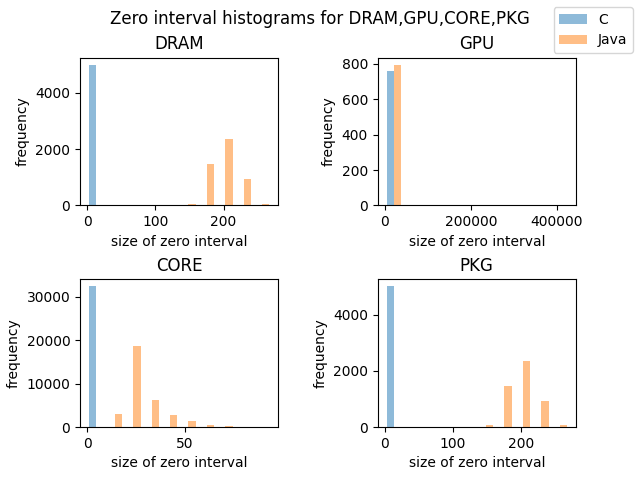
\includegraphics[width=17cm,height=17cm,keepaspectratio]{AsyncMonitorCompares/zero-intervals.png}
    	\caption{"Zero Intervals" histogram for each power domain, compared AsyncEnergyMonitorCSide and AsyncEnergyMonitorJavaSide}
    	\label{fig:xalan-PKG-Time-scatter}
    \end{figure}

\subsubsection{Average Sample Energy}
    Average nonzero energy sample for the CSide monitor and the JavaSide monitor. Looks like the C side monitor
    has higher energy samples, probably because C sampling has lower overhead??

    \begin{figure}[H]
    	\centering
    	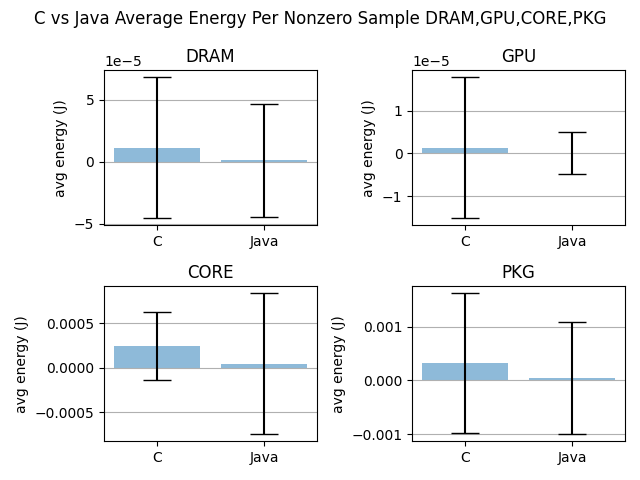
\includegraphics[width=17cm,height=17cm,keepaspectratio]{AsyncMonitorCompares/avg-nonzero-energy-read.png}
    	\caption{Avg nonzero energy read in one sample per each power domain, compared AsyncEnergyMonitorCSide and AsyncEnergyMonitorJavaSide}
    	\label{fig:xalan-PKG-Time-scatter}
    \end{figure}
    
\section{All of my Async Monitor - Related Code}
    My intention behind the code is that you'd use an object of the abstract class AsyncEnergyMonitor, and initialize it to be one of the sub-classes, CSide and JavaSide. So you'd do \texttt{AsyncEnergyMonitor m = new AsyncEnergyMonitorJavaSide()} or \texttt{AsyncEnergyMonitor m = new AsyncEnergyMonitorCSide()}. All of the core utilities
    are defined or declared in the top-level abstract class, so you can use them "interchangeably" with no difference after they've been declared. You can see this
    in the sample main() driver for AsyncEnergyMonitor.java. It picks whether to initialize the AsyncEnergyMonitor as a CSide or JavaSide object based on command line arguments, and then
    the rest of the main driver's functionality works regardless of what kind it was instantiated as.
    
\subsection{AsyncEnergyMonitor.java}
    \begin{framed}
        \lstset{language=java}
        \lstinputlisting[tabsize=2]{java-src/AsyncEnergyMonitor.java}
    \end{framed}
\subsection{AsyncEnergyMonitorJavaSide.java}
    \begin{framed}
        \lstset{language=java}
        \lstinputlisting[tabsize=2]{java-src/AsyncEnergyMonitorJavaSide.java}
    \end{framed}
\subsection{AsyncEnergyMonitorCSide.java}
    \begin{framed}
        \lstset{language=java}
        \lstinputlisting[tabsize=2]{java-src/AsyncEnergyMonitorCSide.java}
    \end{framed}
\subsection{All of the C Side Code Related to AsyncEnergyMonitorCSide}
    \subsubsection{JNI Wrapper Calls}
        \begin{framed}
            \lstset{language=C}
            \lstinputlisting[tabsize=2]{native-src/jni-exports/AsyncEnergyMonitor.c}
        \end{framed}
    \subsubsection{AsyncEnergyMonitor.h}
        \begin{framed}
            \lstset{language=C}
            \lstinputlisting[tabsize=2]{native-src/just-c/AsyncEnergyMonitor.h}
        \end{framed}
    \subsubsection{AsyncEnergyMonitor.c}
        \begin{framed}
            \lstset{language=C}
            \lstinputlisting[tabsize=2]{native-src/just-c/AsyncEnergyMonitor.c}
        \end{framed}
    Different CSide Data Storage Methods for the AsyncEnergyMonitor
    \begin{itemize}
        \item CSideDataStorage.h
            \begin{framed}
                \lstset{language=C}
                \lstinputlisting[tabsize=2]{native-src/just-c/CSideDataStorage.h}
            \end{framed}
        \item CSideDataStorage.c
            \begin{framed}
                \lstset{language=C}
                \lstinputlisting[tabsize=2]{native-src/just-c/CSideDataStorage.c}
            \end{framed}
    \end{itemize}
    

\section{Memory Footprint}
\subsection{Dacapo runs}
Separate tables because we don't really need to compare across all benchmarks, right? Just for different implementations
within each benchmark.

These results are so inconsistent. I don't know what to make of them. Maybe the memory monitor is bad? Mention the (very
occasional) negative values.

Results are aggregate data for all iterations, then subtract \texttt{(monitoring memory with jRAPL) - 
(monitoring memory without jRAPL)} and find the \% difference

\subsubsection{avrora} xxx
    \begin{tabular}{lrrr}
\toprule
{} &  c-linklist &       java &  c-dynamicarray \\
\midrule
avg            &  -22.990984 &  12.034742 &      -15.830842 \\
median\_median  &  -10.563653 &  13.782955 &       -8.024055 \\
average\_median &  -19.341514 &  15.763736 &      -10.116443 \\
global\_min     &   28.378842 &   1.963232 &       12.426157 \\
global\_max     &   -5.205987 &   4.456180 &       -0.754121 \\
avg\_min        &   -7.950443 &  23.166882 &       -9.060579 \\
avg\_max        &   -3.235414 &   3.962927 &       -0.400157 \\
\bottomrule
\end{tabular}

\subsubsection{fop} xxx
    \begin{tabular}{lrrr}
\toprule
{} &  c-dynamicarray &  c-linklist &       java \\
\midrule
avg            &       14.753119 &    3.501001 & -48.453790 \\
median\_median  &       39.205198 &    3.225860 &  -8.999937 \\
average\_median &       10.781817 &    0.271204 & -39.496834 \\
global\_min     &        1.156911 &    0.031209 &   7.017655 \\
global\_max     &        4.322920 &    1.549695 & -38.407106 \\
avg\_min        &       18.662056 &    5.171121 & -56.592499 \\
avg\_max        &       -1.055778 &    0.174332 &  -6.617855 \\
\bottomrule
\end{tabular}

\subsubsection{batik} xxx
    \begin{tabular}{lrrr}
\toprule
{} &       java &  c-linklist &  c-dynamicarray \\
\midrule
avg            &  22.696487 &    2.263102 &       -2.863462 \\
median\_median  &  32.394356 &    9.741842 &       10.559384 \\
average\_median &  25.239511 &    5.405493 &        3.816657 \\
global\_min     &  -9.511461 &  -12.870456 &      -14.141959 \\
global\_max     &  11.693007 &   11.381544 &       -4.696505 \\
avg\_min        &  11.007479 &   -5.950056 &      -13.815936 \\
avg\_max        &  49.583542 &   20.563133 &       -2.033528 \\
\bottomrule
\end{tabular}

\subsubsection{jython} xxx
    \begin{tabular}{lrrr}
\toprule
{} &  c-dynamicarray &       java &  c-linklist \\
\midrule
avg            &        6.788263 &  -1.608247 &   16.832893 \\
median\_median  &       42.390677 &   3.818920 &   46.461562 \\
average\_median &       13.382782 &   5.761306 &   26.412757 \\
global\_min     &       -1.554486 & -15.215190 &   13.329089 \\
global\_max     &        0.651906 &   1.350214 &   -0.952107 \\
avg\_min        &        7.319009 &  -3.782517 &   12.175450 \\
avg\_max        &        8.809611 &  26.179508 &   -6.128205 \\
\bottomrule
\end{tabular}

\subsubsection{luindex} xxx
    \begin{tabular}{llll}
\toprule
{} &               c-linklist &            c-dynamicarray &                    java \\
\midrule
avg            &  (-18.7235, -6815349.27) &  (-16.8957, -6150011.053) &  (8.6028, 3131420.8889) \\
median\_median  &    (-4.5279, -1280998.0) &       (4.3239, 1223284.0) &  (-11.7798, -3332676.0) \\
average\_median &    (-9.6729, -3181911.0) &     (-7.8012, -2566208.0) &   (-4.6957, -1544654.0) \\
global\_min     &      (-1.886, -528432.0) &    (-11.8334, -3315552.0) &  (-10.9234, -3060592.0) \\
global\_max     &     (-1.7092, -128920.0) &        (-0.438, -33040.0) &     (-0.3884, -29296.0) \\
avg\_min        &  (-18.4261, -11427936.0) &   (-17.8035, -11041808.0) &     (9.4147, 5839016.0) \\
avg\_max        &         (0.161, 11654.0) &         (0.7979, 57772.0) &       (1.857, 134452.0) \\
\bottomrule
\end{tabular}

\subsubsection{xalan} xxx
    \begin{tabular}{llll}
\toprule
{} &                       java &                 c-linklist &             c-dynamicarray \\
\midrule
avg            &  (-4.3625, -19994764.5089) &  (27.0189, 123837971.8574) &  (-6.3078, -28910824.0142) \\
median\_median  &     (-4.2961, -18081792.0) &     (-7.0297, -29587182.0) &     (-5.5516, -23366068.0) \\
average\_median &     (-5.3024, -23017416.0) &      (20.5324, 89129655.0) &     (-8.4153, -36530110.0) \\
global\_min     &     (-3.4884, -32727832.0) &    (-10.5263, -98758168.0) &        (0.2279, 2138040.0) \\
global\_max     &         (4.2021, 186472.0) &          (2.0045, 88952.0) &       (24.2762, 1077288.0) \\
avg\_min        &      (-4.096, -41232940.0) &     (39.1272, 393880380.0) &     (-1.8685, -18809892.0) \\
avg\_max        &         (6.8654, 278936.0) &         (6.0701, 246624.0) &        (14.4263, 586126.0) \\
\bottomrule
\end{tabular}

\subsubsection{h2} xx
    \begin{tabular}{lrr}
\toprule
{} &       java &  c-dynamicarray \\
\midrule
avg            &  11.544994 &       -0.761889 \\
median\_median  &  11.274583 &        2.177392 \\
average\_median &   9.478633 &       -2.889813 \\
global\_min     &  19.925900 &        2.378511 \\
global\_max     &   0.189647 &        0.005679 \\
avg\_min        &  13.520432 &       -2.895048 \\
avg\_max        &   0.546450 &        0.183347 \\
\bottomrule
\end{tabular}

\subsubsection{lusearch} xx
    \begin{tabular}{lrrr}
\toprule
{} &  c-linklist &        java &  c-dynamicarray \\
\midrule
avg            &   11.348035 &   11.689136 &        6.938515 \\
median\_median  &   18.329207 &    0.556986 &        8.719691 \\
average\_median &   13.787226 &    8.531274 &        7.370324 \\
global\_min     &    4.488640 &   -2.080764 &       -2.462438 \\
global\_max     &    0.872693 &    3.343817 &        0.405197 \\
avg\_min        &    0.806307 &   11.149241 &       -0.281267 \\
avg\_max        & -246.328405 & -247.556465 &     -246.335929 \\
\bottomrule
\end{tabular}

\subsubsection{zxing} xx
    \begin{tabular}{llll}
\toprule
{} &          c-dynamicarray &                    java &              c-linklist \\
\midrule
avg            &  (2.1951, 4134357.3196) &  (0.9214, 1735351.9526) &  (3.9253, 7393137.6379) \\
median\_median  &   (-2.2595, -4036628.0) &     (2.6172, 4675690.0) &   (-2.5914, -4629582.0) \\
average\_median &   (-1.5272, -2705577.0) &     (3.4806, 6166286.0) &     (0.6991, 1238622.0) \\
global\_min     &    (6.2281, 28514976.0) &    (5.9169, 27090008.0) &    (6.6973, 30663048.0) \\
global\_max     &       (2.6989, 78256.0) &      (5.6162, 162848.0) &       (1.7939, 52016.0) \\
avg\_min        &    (2.8539, 13864754.0) &    (4.4813, 21770612.0) &    (3.0905, 15014010.0) \\
avg\_max        &        (2.454, 71030.0) &      (5.2478, 151896.0) &       (1.8055, 52260.0) \\
\bottomrule
\end{tabular}

\subsubsection{h2o} xx
    \begin{tabular}{lrrr}
\toprule
{} &      java &  c-dynamicarray &  c-linklist \\
\midrule
avg            &  7.965396 &       -5.276288 &    4.574933 \\
median\_median  &  3.081788 &      -20.089399 &    2.252259 \\
average\_median &  8.238086 &       -5.829436 &    8.047533 \\
global\_min     &  9.307872 &      -14.283249 &    2.491613 \\
global\_max     &  4.154166 &       -0.373717 &    0.064644 \\
avg\_min        &  9.334081 &       -6.589612 &   11.094129 \\
avg\_max        &  1.161256 &        0.699436 &   -0.184486 \\
\bottomrule
\end{tabular}

\subsubsection{eclipse} xx
    \begin{tabular}{llll}
\toprule
{} &                c-linklist &                     java &           c-dynamicarray \\
\midrule
avg            &  (-0.9156, -4599310.9884) &  (4.0881, 20534937.2432) &  (2.7898, 14013062.9081) \\
median\_median  &       (0.6972, 3496252.0) &      (3.201, 16052414.0) &     (3.2102, 16098372.0) \\
average\_median &       (1.8944, 9439314.0) &     (4.5652, 22747559.0) &     (3.2205, 16047018.0) \\
global\_min     &    (-4.1612, -37979336.0) &   (-6.8661, -62667696.0) &    (-0.3035, -2770392.0) \\
global\_max     &      (10.5672, 8695552.0) &    (14.0544, 11565120.0) &      (4.2668, 3511104.0) \\
avg\_min        &      (3.0222, 29061762.0) &   (-5.5033, -52920764.0) &     (6.5192, 62690096.0) \\
avg\_max        &       (-1.48, -1131866.0) &      (2.4816, 1897806.0) &      (-1.224, -936080.0) \\
\bottomrule
\end{tabular}

\subsubsection{tradebeans} xx
    \begin{tabular}{llll}
\toprule
{} &                     java &           c-dynamicarray &              c-linklist \\
\midrule
avg            &  (5.1286, 28960279.5019) &  (3.0239, 17075392.3684) &  (3.8327, 21642454.143) \\
median\_median  &     (5.4019, 28938258.0) &     (3.1155, 16689776.0) &    (4.1732, 22356010.0) \\
average\_median &     (6.0504, 32407995.0) &     (3.5891, 19224075.0) &    (3.9897, 21369865.0) \\
global\_min     &   (15.2268, 159072024.0) &   (11.3878, 118967192.0) &    (9.1547, 95637680.0) \\
global\_max     &      (0.5586, 1039872.0) &       (0.0755, 140496.0) &      (0.0656, 122040.0) \\
avg\_min        &     (5.5244, 64677464.0) &     (3.7717, 44157602.0) &    (2.9203, 34189264.0) \\
avg\_max        &    (36.2691, 38179394.0) &    (76.7771, 80820896.0) &   (38.1944, 40206086.0) \\
\bottomrule
\end{tabular}

\subsubsection{tomcat} x
    \begin{tabular}{llll}
\toprule
{} &            c-dynamicarray &                    java &               c-linklist \\
\midrule
avg            &  (11.9506, 18230031.5696) &  (-0.9393, -1432798.16) &    (1.337, 2039528.2917) \\
median\_median  &     (20.9717, 25152276.0) &      (0.7904, 947988.0) &      (2.4482, 2936256.0) \\
average\_median &     (20.9201, 24994008.0) &       (0.0442, 52793.0) &      (1.1319, 1352357.0) \\
global\_min     &     (-0.6042, -2826664.0) &  (-3.3998, -15905888.0) &  (-13.2944, -62197248.0) \\
global\_max     &          (0.408, 77024.0) &       (0.896, 169128.0) &       (0.6736, 127160.0) \\
avg\_min        &     (-0.5918, -2847078.0) &   (-0.7171, -3450292.0) &   (-4.0893, -19674824.0) \\
avg\_max        &         (0.3159, 56352.0) &      (0.8728, 155716.0) &        (0.4783, 85338.0) \\
\bottomrule
\end{tabular}

\subsubsection{cassandra} x
    \begin{tabular}{llll}
\toprule
{} &              c-linklist &            c-dynamicarray &                   java \\
\midrule
avg            &  (9.9359, 8980398.7732) &  (12.7405, 11515300.2187) &  (13.537, 12235163.14) \\
median\_median  &     (3.2085, 2730740.0) &       (7.8899, 6715152.0) &     (8.499, 7233592.0) \\
average\_median &    (10.1917, 8788248.0) &       (7.3162, 6308764.0) &    (7.4323, 6408854.0) \\
global\_min     &   (12.1211, 13539600.0) &       (5.6473, 6308168.0) &    (6.6424, 7419752.0) \\
global\_max     &       (0.1334, 76032.0) &         (0.0655, 37344.0) &   (-0.3031, -172800.0) \\
avg\_min        &   (11.0816, 13717244.0) &     (-1.7151, -2123056.0) &    (1.4322, 1772814.0) \\
avg\_max        &      (0.2158, 111702.0) &         (0.0988, 51162.0) &      (0.1709, 88454.0) \\
\bottomrule
\end{tabular}

\subsubsection{sunflow} x
    \begin{tabular}{llll}
\toprule
{} &                      java &               c-linklist &            c-dynamicarray \\
\midrule
avg            &  (-0.9879, -4631947.8975) &  (4.6891, 21985517.0939) &  (13.0854, 61352695.4562) \\
median\_median  &       (1.4055, 5719914.0) &     (4.8105, 19576984.0) &     (16.4754, 67049734.0) \\
average\_median &      (2.6336, 10726119.0) &     (2.9576, 12045696.0) &     (15.7632, 64200147.0) \\
global\_min     &  (-15.3376, -190301008.0) &  (-8.7616, -108709280.0) &    (-3.7308, -46290320.0) \\
global\_max     &         (1.522, 297768.0) &       (0.5876, 114952.0) &        (0.5427, 106168.0) \\
avg\_min        &   (-14.128, -187563474.0) &   (-5.3441, -70948860.0) &      (3.5985, 47773078.0) \\
avg\_max        &        (1.2425, 242962.0) &        (0.4296, 84010.0) &         (0.3387, 66230.0) \\
\bottomrule
\end{tabular}

\subsubsection{biojava} x
    \begin{tabular}{lrrr}
\toprule
{} &       java &  c-dynamicarray &  c-linklist \\
\midrule
avg            &   3.145939 &        5.108169 &    1.398809 \\
median\_median  &   0.002372 &        5.386789 &    1.548125 \\
average\_median &   2.159418 &        5.358550 &    1.202894 \\
global\_min     & -12.219386 &       -6.099006 &  -12.421726 \\
global\_max     &  15.669497 &        2.248432 &    2.311211 \\
avg\_min        &   2.846762 &        3.883716 &   -0.047027 \\
avg\_max        &  17.816112 &        2.733910 &    2.818863 \\
\bottomrule
\end{tabular}

\subsubsection{pmd} x
    \begin{tabular}{lrrr}
\toprule
{} &      java &  c-dynamicarray &  c-linklist \\
\midrule
avg            & -0.727953 &       -0.044044 &   -3.971566 \\
median\_median  & -0.191747 &        0.884891 &   -3.553471 \\
average\_median & -1.334457 &        0.503858 &   -4.182274 \\
global\_min     &  0.289310 &        0.156184 &   -5.132336 \\
global\_max     &  0.355585 &        0.054602 &    0.047014 \\
avg\_min        &  0.141190 &        0.042842 &   -1.747980 \\
avg\_max        &  0.399434 &        0.070033 &    0.001174 \\
\bottomrule
\end{tabular}

\subsubsection{jme} x
    \begin{tabular}{llll}
\toprule
{} &            c-dynamicarray &                    java &              c-linklist \\
\midrule
avg            &  (-5.9823, -8223332.1443) &  (3.8386, 5276613.2424) &    (0.9123, 1254073.48) \\
median\_median  &      (10.7172, 2716788.0) &    (13.9688, 3541064.0) &     (4.1141, 1042916.0) \\
average\_median &       (9.0819, 2384244.0) &    (11.4863, 3015456.0) &      (1.0825, 284184.0) \\
global\_min     &  (-12.9885, -171018072.0) &  (-1.4307, -18837336.0) &  (-0.9547, -12570760.0) \\
global\_max     &         (0.1776, 28448.0) &      (1.4193, 227328.0) &       (0.1764, 28256.0) \\
avg\_min        &    (-6.5759, -87786996.0) &    (1.8123, 24193622.0) &    (1.5697, 20955470.0) \\
avg\_max        &         (0.5652, 71086.0) &      (1.8159, 228392.0) &       (0.4769, 59986.0) \\
\bottomrule
\end{tabular}

\subsubsection{graphchi} x
    \begin{tabular}{lrrr}
\toprule
{} &       java &  c-linklist &  c-dynamicarray \\
\midrule
avg            &   0.320569 &   -0.757283 &        1.683155 \\
median\_median  &  -2.741298 &   -0.988912 &       -3.469857 \\
average\_median &   0.002802 &   -0.809347 &        0.921065 \\
global\_min     & -27.464651 &    3.210571 &        1.767143 \\
global\_max     &   2.449260 &   -0.792516 &        1.116776 \\
avg\_min        &  -3.970983 &   -2.008806 &        0.138969 \\
avg\_max        &   3.036588 &  231.369337 &        1.505898 \\
\bottomrule
\end{tabular}

\subsubsection{tradesoap} x
    \begin{tabular}{lrrr}
\toprule
{} &  c-linklist &       java &  c-dynamicarray \\
\midrule
avg            &   -6.178576 &   7.175885 &       -2.784059 \\
median\_median  &   -4.682000 &   6.241045 &       -2.977609 \\
average\_median &   -5.079088 &   6.254456 &       -2.233216 \\
global\_min     &   -0.279456 &  18.810754 &       14.731709 \\
global\_max     &    1.142778 &   1.871280 &        0.465544 \\
avg\_min        &  -14.819571 &   5.277596 &       -5.120683 \\
avg\_max        &    0.718773 &   1.273663 &        0.430002 \\
\bottomrule
\end{tabular}

    
\subsection{Object Sample vs Primitive Array Sample}
Used the classmexer agent provided at https://javamex.com/classmexer/

It uses instrumentation to get the memory usage of an object, so the object header
(12 bytes) and the size of all of its fields. I made sure to ask for deep memory
usage, so if its fields are non-primitive types, we also get the number of bytes
in the entire object, not just of the reference stored in the top level object. Java
object sizes are padded up to the next multiple of 8. Units are bytes.

Below is the output of my test program, where I took an array sample and an object
sample, and got the deep memory use of each.
\begin{verbatim}










For raw stamp sample:
  primitive sample: 48 bytes
  object sample: 96 bytes
    [1164.4618, 184.5864, 4048.8065, 11751.1702]
    1164.4625,184.5864,4048.8231,11751.1893,1619625664691708

For diff sample (over a 100ms delay):
  primitive sample: 48 bytes
  object sample: 96 bytes
    [0.017399999999952342, 0.0, 0.16520000000036816, 0.30240000000048894]
    0.0235,0.0096,0.0237,0.1486,101030
    
    
    
\end{verbatim}

These results are on my computer, since Jolteon currently has my other experiments
running, so we'd get other values since it's a 2socket/3power-domain machine, as opposed to my 1socket/4power-domain machine.

Math checks out. Primitive sample is header (12 bytes) + 4 doubles (32 bytes) =
44, rounded up to 48.
Object sample is header (12) + primitive sample (44 +4padding) + Instant(12 + 8 + 8) = 88, round up to 96.

\textbf{66\% percent difference} in sizes of these implementations

\subsection{deprecated experiment}
    The only memory footprint test I did was seeing if there was a remarkable difference between the AsyncEnergyMonitor
    storing double[]s as energy samples or EnergyStats objects. However, Timur and I decided that it actually made
    the most sense to just store raw energy Strings returned directly from the native interface. There's no overhead
    that we'd have to deal with for parsing it while we're monitoring, and it may be that these end up getting written
    to a file anyways, so we'd have to turn the back into Strings. So instead, I just made some functionality to ask
    for samples as Objects or Arrays if we actually need to take them out of the AsyncEnergyMonitor during the code. But
    internally they're just strings. So the point of this specific experiment is over. Here are the results, though.

    What I did was ran two versions of the AsyncEnergyMonitorJavaSide, one which internally stored double[]s for
    energy samples, the other one which stored EnergyStats objects. Then I used an AsyncMemoryMonitor that I made.
    The memory monitor is the same type of thing as the energy monitor. Start a thread, collect memory samples at a
    set millisecond sampling rate. The memory monitor collected throughout the lifetime of the energymonitors as
    they grew in memory while collecting.
    
    I still have the memory monitor for other purposes, though.

    \begin{figure}[H]
    	\centering
    	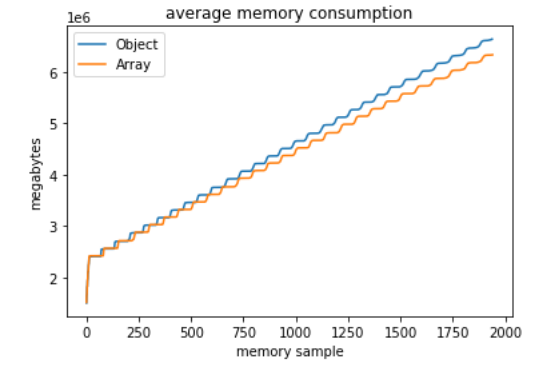
\includegraphics[width=10cm,height=10cm,keepaspectratio]{MemoryFootprint/ArrayVsObjectStorage_(deprecated)/average_memory_consumption.png}
    	\caption{Memory growth of the Object storage based and Array storage based (now deprecated) implementations
    	of AsyncEnergyMonitorJavaSide}
    	\label{fig:avg-sample-PKG}
    \end{figure}
    
    \begin{figure}[H]
    	\centering
    	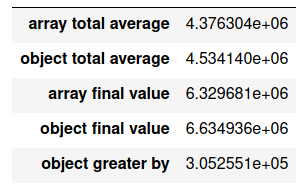
\includegraphics[width=10cm,height=10cm,keepaspectratio]{MemoryFootprint/ArrayVsObjectStorage_(deprecated)/memory_consumption_table.png}
    	\caption{Some stats about the memory footprint of each implementation. These units are in bytes}
    	\label{fig:avg-sample-PKG}
    \end{figure}

    The object sample implementation was about .3 MB larger than the array based one, after running and growing
    for 20 seconds.


\section{Jolteon Stuff}
    All of these tests are done on the Jolteon server. Jolteon supports DRAM, CORE, and PKG, but \emph{not} GPU

    \subsection{JNI Overhead (difference between JNI calls timed from Java and from C)}
    These were done on Jolteon server with Java Microbenchmark Harness (JMH).
    
    \textbf{JMH Parameters:} 10 second trials, ran as many times as possible in the 10 second period. 1 fork, 5 warmup iterations, 10 measurement iterations. Results are cumulative (not averaged) for the 10 iterations, not including the warmups.
    
    We used our own timestamping as opposed to JMH's \texttt{Mode.AverageTime} utility because 1) we wanted individual readings to plot all of them as opposed to just the average and 2) we had to timestamp stuff on the C side, which there was no way JMH could do for us. Java timestamps were \texttt{Instant.now()} and C timestamps where \texttt{gettimeofday()}. Runtimes were stored in a \texttt{HashMap<Long,Long>} as a histogram. All measurements are in microseconds unless otherwise specified. 
    
    The graphs below are histograms. X axis is the microsecond runtimes, Y axis is how many readings we got
    for that runtime. Crazy high values (more than 3 standard deviations from the mean) are removed because they are relatively few and that stretch the graph and make it illegible. But we still captured
    them in the Python script, because they're probably important information and intend to render them somehow.

    The Java runtimes for EnergyStatCheck are way higher and more volatile...this is weird because when we were doing our original non-JMH runtime drivers,
    there was a pretty negligible difference between CSide and JavaSide runtime (see the first graph in Section 2, Runtime Tests). I don't know if it's because we wrote the JavaSide benchmarks poorly, but I couldn't find anything egregiously wrong. Maybe it's the magic of JMH giving us an actual look at what a real environment would be, and the original drivers we wrote were just prone to unrealistic optimization? Maybe it's because a String is actually being brought across the Java Native Interface; ProfileInit and ProfileDealloc are void functions. So the JVM could've realized that we weren't actually using the String and optimized out the conversion from a C JNIEXPORT String to a Java String. I'm not sure though, definitely something to look at more.
    
    
    \begin{figure}[H]
	    \centering
	    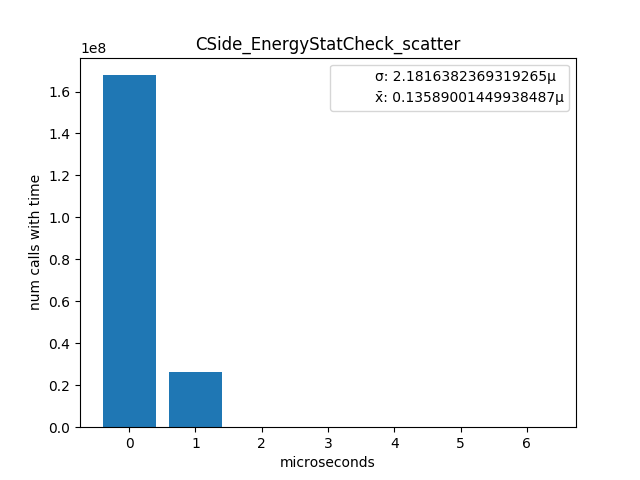
\includegraphics[width=10cm,height=10cm,keepaspectratio]{jolteon/jmh/jni-overhead/CSide_EnergyStatCheck_scatter.png}
	    \caption{Runtime for EnergyStatCheck on CSide}
	    \label{fig:jolteon-jmh-runtime-energystatcheck-c}
    \end{figure}
    \begin{figure}[H]
	    \centering
	    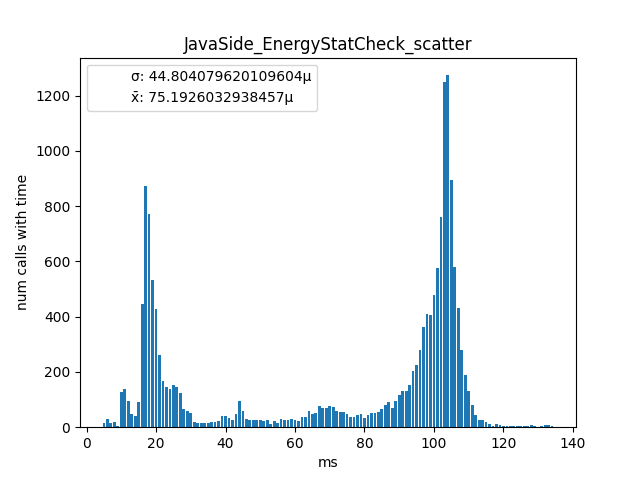
\includegraphics[width=10cm,height=10cm,keepaspectratio]{jolteon/jmh/jni-overhead/JavaSide_EnergyStatCheck_scatter.png}
	    \caption{Runtime for EnergyStatCheck on JavaSide}
	    \label{fig:jolteon-jmh-runtime-energystatcheck-java}
    \end{figure}
    
    \begin{figure}[H]
	    \centering
	    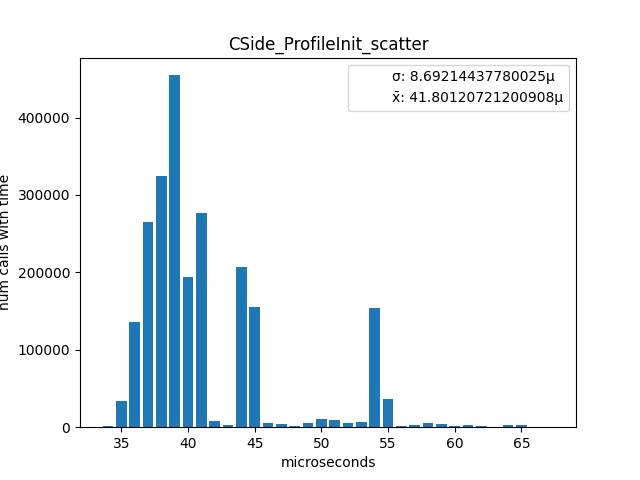
\includegraphics[width=10cm,height=10cm,keepaspectratio]{jolteon/jmh/jni-overhead/CSide_ProfileInit_scatter.png}
	    \caption{Runtime for ProfileInit on CSide}
	    \label{fig:jolteon-jmh-runtime-profileinit-c}
    \end{figure}
    \begin{figure}[H]
	    \centering
	    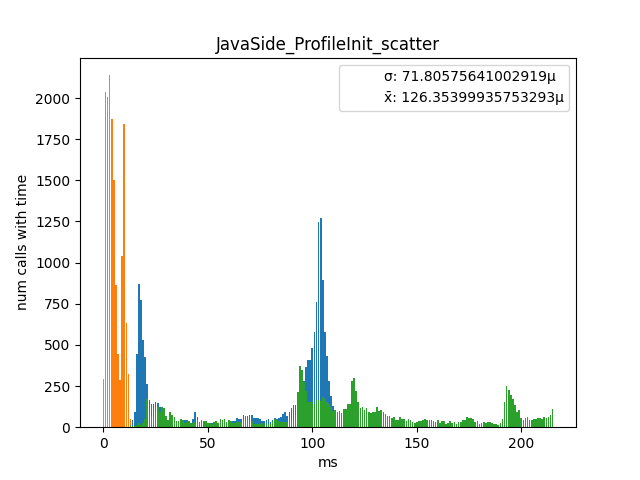
\includegraphics[width=10cm,height=10cm,keepaspectratio]{jolteon/jmh/jni-overhead/JavaSide_ProfileInit_scatter.png}
	    \caption{Runtime for ProfileInit on JavaSide}
	    \label{fig:jolteon-jmh-runtime-profileinit-java}
    \end{figure}

    \begin{figure}[H]
	    \centering
	    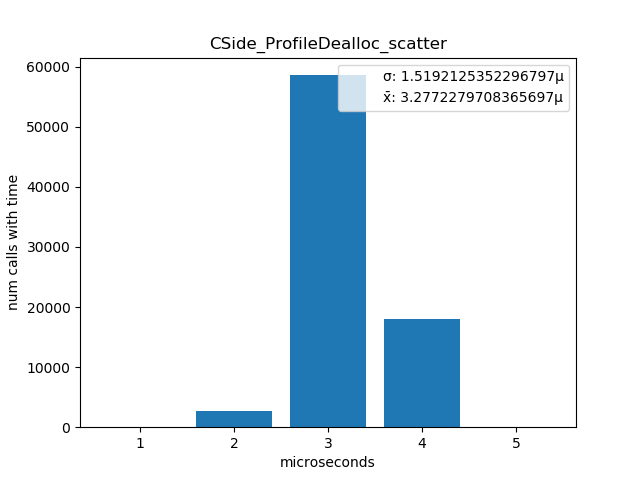
\includegraphics[width=10cm,height=10cm,keepaspectratio]{jolteon/jmh/jni-overhead/CSide_ProfileDealloc_scatter.png}
	    \caption{Runtime for ProfileDealloc on CSide}
	    \label{fig:jolteon-jmh-runtime-profileDealloc-c}
    \end{figure}
    \begin{figure}[H]
	    \centering
	    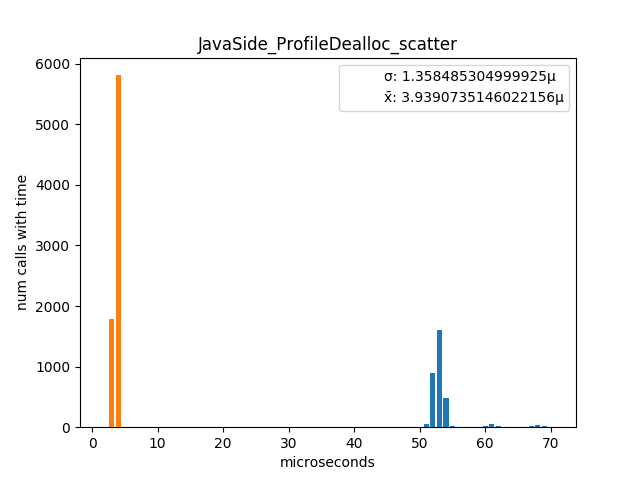
\includegraphics[width=10cm,height=10cm,keepaspectratio]{jolteon/jmh/jni-overhead/JavaSide_ProfileDealloc_scatter.png}
	    \caption{Runtime for ProfileDealloc on JavaSide}
	    \label{fig:jolteon-jmh-runtime-profileDealloc-java}
    \end{figure}
    

    \subsection{Time to read one MSR register}
    How long it takes to read one individual MSR register to get the RAPL counter. It's worth noting that we're not actually accessing the register, but a type of file that Linux provides as an interface where every 8 bytes internally maps to the actual hardware register. Just good to keep that distinction in mind.
    
    It's all hovering around one microsecond, with occasional relatively-high values. Values greater than 3 standard deviations weren't plotted because it makes the graph illegible, but we still captured them
    in the Python script and intend to represent them somehow, because it's still probably good to know
    that we'll very occasionally get super high runtimes.
    
    We used our own timestamping as opposed to JMH's \texttt{Mode.AverageTime} utility because 1) we wanted individual readings to plot all of them as opposed to just the average and 2) we had to timestamp stuff on the C side, which there was no way JMH could do for us. Java timestamps were \texttt{Instant.now()} and C timestamps where \texttt{gettimeofday()}. Runtimes were stored in a \texttt{HashMap<Long,Long>} as a histogram. All measurements are in microseconds unless otherwise specified. 
    
    Graphs below are histograms. X axis is the runtime, Y axis is how many readings we found at that runtime.
    
    \begin{figure}[H]
	    \centering
	    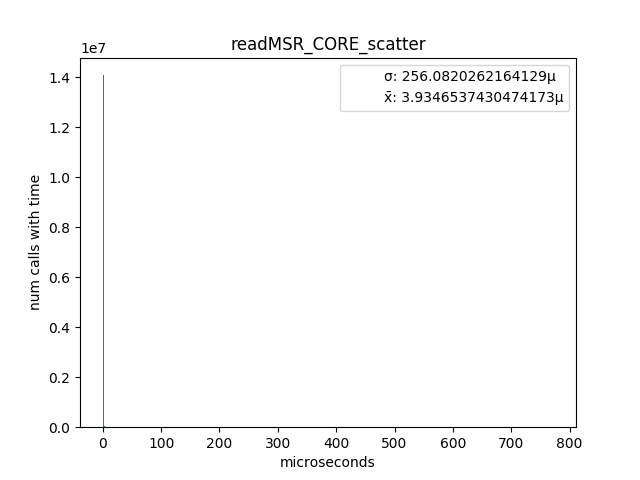
\includegraphics[width=10cm,height=10cm,keepaspectratio]{jolteon/jmh/readmsr-runtime/readMSR_CORE_scatter.png}
	    \caption{Runtime to read MSR for CORE RAPL counter}
	    \label{fig:CORE-rapl-counter}
    \end{figure}
    
    \begin{figure}[H]
	    \centering
	    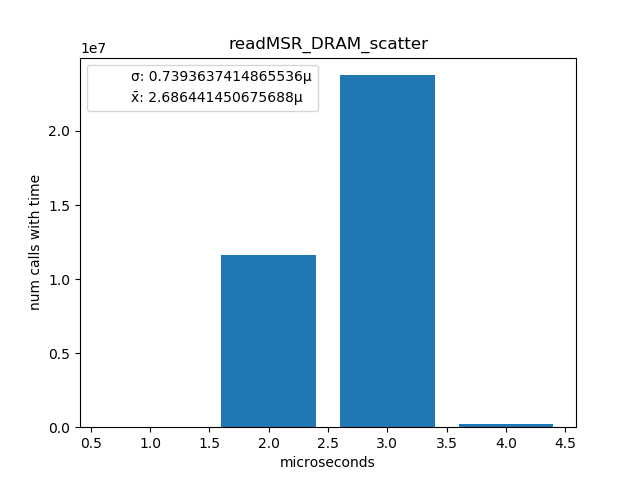
\includegraphics[width=10cm,height=10cm,keepaspectratio]{jolteon/jmh/readmsr-runtime/readMSR_DRAM_scatter.png}
	    \caption{Runtime to read MSR for DRAM RAPL counter}
	    \label{fig:DRAM-rapl-counter}
    \end{figure}
    
    \begin{figure}[H]
	    \centering
	    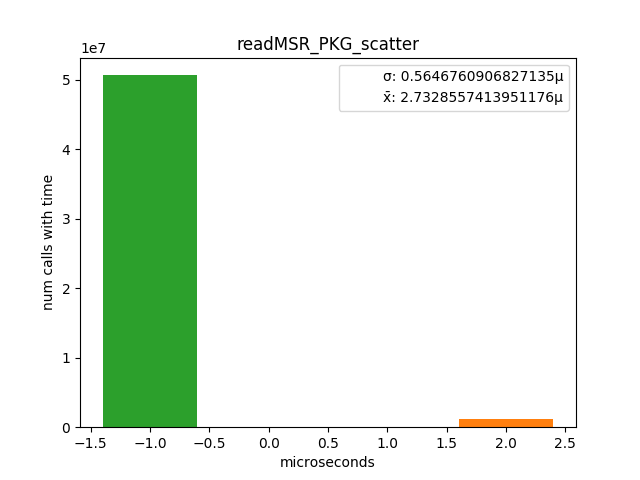
\includegraphics[width=10cm,height=10cm,keepaspectratio]{jolteon/jmh/readmsr-runtime/readMSR_PKG_scatter.png}
	    \caption{Runtime to read MSR for PKG RAPL counter}
	    \label{fig:PKG-rapl-counter}
    \end{figure}
    
    %\begin{figure}[H]
	%    \centering
	%    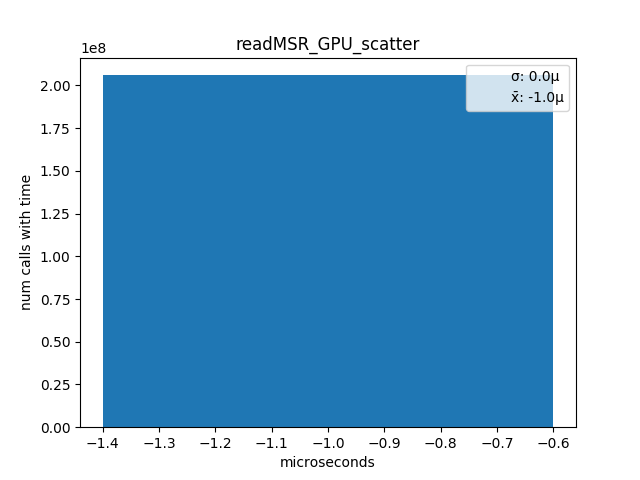
\includegraphics[width=10cm,height=10cm,keepaspectratio]{jolteon/jmh/readmsr-runtime/readMSR_GPU_scatter.png}
	%    \caption{Runtime to read MSR for GPU RAPL counter}
	%    \label{fig:GPU-rapl-counter}
    %\end{figure}
    

\end{document}



























